%% This is annot.tex.
%% 
%% You'll need to change the title and author fields to reflect your
%% information.
%%
%% Author: Titus Barik (titus@barik.net)
%% Homepage: http://www.barik.net/sw/ieee/
%% Reference: http://www.ctan.org/tex-archive/info/simplified-latex/

\documentclass [11pt]{article}
\usepackage[dvipsnames]{xcolor}
\usepackage{graphicx}% Include figure files
\usepackage[spanish]{babel}
\selectlanguage{spanish}
\usepackage[utf8]{inputenc}
\usepackage{upgreek}

\usepackage{mathtools}
\usepackage{braket}

\usepackage{xcolor}

\title{Tesis \\\medskip segundo borrador}
\author{Daniel Sucerquia Gaviria (daniel.sucerquia@udea.edu.co)\\Universidad de Antioquia Technology}

\begin{document}
\maketitle

{\Large \bf Notación}\\

{\color{red} No entiendo}\\
{\color{blue} Creo que es así, pero tengo que aclararlo mejor para estar
seguro}\\
{\color{Brown} corrección revisada}
\section{Separación de la dinámica de electrones y núcleos con la aproximación Born-Oppenheimer}
%Olga: te voy a introducir unos titulos para las secciones
El Hamiltoniano que se comienza considerando es:
%1
\begin{equation}
    {\hat H}_{tot}={\hat T}_n+{\hat T}_e+{\hat V}_{ne}+{\hat V}_{ee}+{\hat V}_{nn}
\end{equation}

Que se puede reescribir como:
%2-4
\begin{eqnarray}
    {\hat H}_{tot} & =  & {\hat T}_n+{\hat H}_e\\
    {\hat H}_e & = & {\hat T}_e+{\hat V}_{ne}+{\hat V}_{ee}+{\hat V}_{nn}
\end{eqnarray}
%Olga: Te aconsejo no uses la descripcion que incluye el centro de masa sino que dejes el operador cinetico de los nucleos como el operador cinetico total donde cada termino es el cinetico con respecto a cada R
$\hat H_e $ es la energía electrónica, y vemos que ésta sólo depende de la posición de los átomos y no de sus momentums. Se va a asumir que existe una solción para el Hamiltoniano electrónico  en las coordenadas de los $b$ electrones ${\bf r}=({\bf r}_1,...,{\bf r}_b)$ y parametrizado con las coordenadas de los $d$ núcleos ${\bf R}=(/{\bf R}_1,...,{\bf R}_d)$. Además, tenemos que el hamiltoniano electrónico es hermítico y por lo tanto puede escogerse como solución una base ortonormal. De manera que:  
%5-6
\begin{eqnarray}
    {\hat H}_e({\bf R}) \Phi_i({\bf r};{\bf R})=\upvarepsilon_i({\bf R}) \Phi_i({\bf r};{\bf R})\\
    \int \Phi_i^*({\bf r};{\bf R})\Phi_j({\bf r};{\bf R})d{\bf r}=\delta_{ij}
\end{eqnarray}

De ésta forma, las funciones de onda se convierten en una base sobre la que se puede expandir la solución del Hamiltoniano total considerando los coeficientes como funciones de la posición de los núcleos:
%7
\begin{equation}
    \Uppsi_k({\bf R},{\bf r})=\sum_{i=1}^{\infty}\upchi_{ik}({\bf R})\Phi_i({\bf r};{\bf R})
\end{equation}
%Olga: Es muy dificil (lease es imposible) de leer esta demonstracion escogiendo la misma letra para todas las funciones de onda (total, de los nucleos y la funcion de onda de los electrones). Te aconsejo que cambies la funcion de onda de los nucleos por \chi y la de los electrones guardes upsi ya que es la que mas escribes y la total puede ser \Phi por ejemplo


Aplicando el hamiltoniano total a esta base, la cual debe ser autofunción (La dependencia de $\upchi_{ik}$ es sólo en ({\bf R}), mientras que la dependencia de $\Phi_i$ es en ({\bf r};{\bf R}), por simplicidad, aquí se evita escribirlas):
%8-10
\begin{eqnarray}
    \hat H_{tot}\Uppsi_k & = & E_k\Uppsi_k\\
    \left({\hat T}_n+{\hat H}_e\right)\left(\sum_{i=1}^{\infty}\upchi_{ik}\Phi_i\right) & = & E_k \left(\sum_{i=1}^{\infty}\upchi_{ik}\Phi_i\right)\\
    \sum_{i=1}^{\infty}\left({\hat T}_n\upchi_{ik}\Phi_i+\upchi_{ik}{\hat H}_e\Phi_i\right) & = & E_k \left(\sum_{i=1}^{\infty}\upchi_{ik}\Phi_i\right)
\end{eqnarray}

Además, $\hat T_n=-\sum_{a}\frac{1}{2M_{a}}\nabla_a^2=\nabla_R^2$, donde nos permitimos definir el nuevo operador $\nabla_R$ aprovechando la linealidad del operador $\nabla_a$, que opera sólo sobre las coordenadas de los iones {\bf R}. De manera que lo que tenemos es:
%11-13
\begin{eqnarray}
    \sum_{i=1}^{\infty}\left({\nabla_R^2}\upchi_{ik}\Phi_i+\upchi_{ik}{\hat H}_e\Phi_i\right) & = & E_k \left(\sum_{i=1}^{\infty}\upchi_{ik}\Phi_i\right)\\
    \sum_{i=1}^{\infty}\left({\nabla_R}\cdot({\nabla_R}\upchi_{ik}\Phi_i+\upchi_{ik}{\nabla_R}\Phi_i)+\upchi_{ik}\upvarepsilon_i\Phi_i\right) & = & E_k \left(\sum_{i=1}^{\infty}\upchi_{ik}\Phi_i\right)\\
    \sum_{i=1}^{\infty}\left(\begin{array}{cc}
         {\nabla_R}^2\upchi_{ik}\Phi_i+2{\nabla_R}\upchi_{ik}\cdot {\nabla_R}\Phi_i+\\
         \upchi_{ik}{\nabla_R}^2\Phi_i+\upvarepsilon_i\upchi_{ik}\Phi_i
    \end{array}\right) & = & E_k \left(\sum_{i=1}^{\infty}\upchi_{ik}\Phi_i\right)
\end{eqnarray}\\

Proyectando sobre el estado $\Phi_j^*$:
\begin{eqnarray*}
    {\nabla_R}^2\upchi_{jk}+\upvarepsilon_j \upchi_{jk}+\sum_{i=1}^{\infty}\left(2{\nabla_R}\upchi_{ik}\cdot\int \Phi_j^*{\nabla_R}\Phi_i d{\bf r}+\upchi_{ik}\int \Phi_j^*{\nabla_R^2}\Phi_i d{\bf r}\right) & = & E_k\upchi_{jk}
\end{eqnarray*}

Utilizando la notación de Dirac para más comodidad en la lectura lo que se tiene es:

\begin{eqnarray*}
    {\nabla_R}^2\upchi_{jk}+\upvarepsilon_j \upchi_{jk}+\sum_{i=1}^{\infty}\left(2{\nabla_R}\upchi_{ik}\cdot\langle\Phi_j|\nabla_R|\Phi_i\rangle+\upchi_{ik}\langle\Phi_j|{\nabla_R^2}|\Phi_i\rangle \right) & = & E_k\upchi_{jk}
\end{eqnarray*}

{\color{red} esto no lo entiendo muy bien: Los dos términos de la sumatoria son respectivamente el primer y segundo {\it elementos del acoplamiento no-adiabático} respectivamente.Éstos términos son relevantes en situaciones donde hay transición de niveles de energía electrónicos como reacciones fotoquímicas.}
En la aproximación adiabática, la forma de la función de onda total está restringida a una superficie electrónica, es decir, se elimina cualquier término de acople (sólo ``sobreviven" los términos donde i=j) \cite{jensen}. {\color{red} Pero eliminan también el término de $2{\nabla_R}\upchi_{ik}\cdot\langle\Phi_j|\nabla_R|\Phi_i\rangle$ y no explican por qué}. Por lo tanto, que lo que se tiene es:
%Olga: Son dos aproximaciones en una. La primera corresponde a tomar un solo termino de la suma en el ansatz para la funcion de onda total (que te sugiero reescribir para que quede clara) esto efectivamente es hacer i=j. La segunda aproximacion es despreciar esas derivadas. El sentido de despreciar esto lo voy a trabajar con Ana y Cristian el proximo Martes en la tarde tomando el ejemplo de una molecula diatomica. Seria bueno que vinieras para aclarar esto.
\begin{eqnarray*}
    {\nabla_R}^2\upchi_{jk}+\upvarepsilon_j \upchi_{jk}+\upchi_{jk}\langle\Phi_j|{\nabla_R^2}|\Phi_j\rangle =  E_k\upchi_{jk}
\end{eqnarray*}

Retomando la definición anterior que se le había dado de $\hat T_n=\nabla_R^2$:

\begin{eqnarray*}
    (\hat T_n+\upvarepsilon_j+\langle\Phi_j|{\nabla_R^2}|\Phi_j\rangle) \upchi_{jk} =  E_k\upchi_{jk}
\end{eqnarray*}

En la aproximación de Born-Oppenheimer (BOA), el término de $\langle\Phi_j|{\nabla_R^2}|\Phi_j\rangle$, conocido como corrección diagonal es ignorado y entonces se obtiene, retomando la notación con las dependencias:

\begin{equation}\label{BOA}
    (\hat T_n+\upvarepsilon_j({\bf R})) \upchi_{jk}({\bf R}) =  E_k\upchi_{jk}({\bf R})
\end{equation}

Que es la forma de la ecuación de Schrödinger. Entonces en la BOA se asume que la dinámica de los núcleos está mediada por una superficie de energía potencial dada por la solución de la ecuación de Schrödinger electrónica. Otra forma de entender conceptualmente la BOA es considerar que los cambios en la dinámica de los electrones y los núcleos se dan sobre escalas de tiempo bastante diferentes, con una diferencia de 3 ordenes de magnitud aproximadamente, al punto de que se pueden solucionar las ecuaciones dinámicas de forma independiente \cite{bransden}.

Nótese que parte de la suposición fundamental de la BOA es la restricción a superficies electrónicas y por eso se despreciaron los términos cruzados más arriba. Físicamente, ésta restricción supone que el movimiento de los iones, no altera el estado de energía de los electrones. Para poder que ésto se mantenga y la BOA siga siendo válida, se debe garantizar que la solución de los niveles de energía electrónica no se aproximen unos a otros para cualquier valor de {\bf R}. Por ejemplo, para el caso de la molécula LiF, existe una solución altamente polarizada representada por una función de onda iónica. Otra solución es la de la molécula disociada en dos átomos neutros. A cortas distancias, la energía de la solución iónica es menor, pero al incrementar la distancia de los núcleos ésta pasa a ser mayor como se ve en la figura \ref{cross}.\\

\begin{figure}[t]
\centering
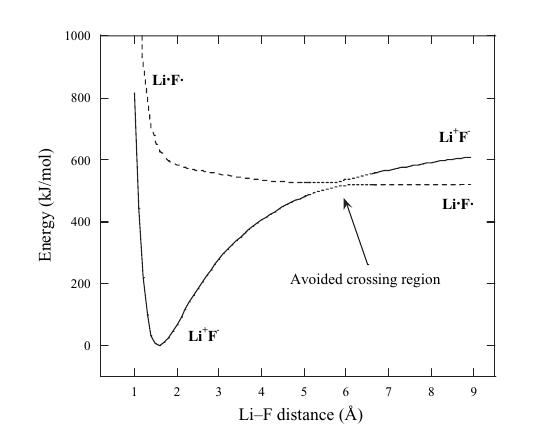
\includegraphics[width=0.8\linewidth]{cross_energy}
\caption{Ejemplo de cruce de energía para la molécula Li-F}
\label{cross}
\end{figure}

Antes de finalizar esta sección, se recuerda el Teorema de Ehrenfest que aborda el problema de la conexión entre las descripciones clasicas y cuanticas \cite{cohen}. Éste, explicitamente remarca que, siendo $\hat A$ el operador de un observable, entonces se cumple que:

\begin{equation}
    \frac{d\langle\hat A\rangle}{dt}=i \langle [\hat H,\hat A]\rangle+\Braket{\frac{\partial\hat A}{\partial t}}
\end{equation}

Aplicando el teorema de Ehrenfest al observable momentum del s-esimo átomo, con el hamiltoniano de la ecuación (\ref{BOA}):

\begin{equation*}
    \frac{d\langle\hat P_s\rangle_{\upchi_{jk}}}{dt}= \frac{i}{\hbar} \langle [\hat T_n+\upvarepsilon_j({\bf R}),\hat P_s]\rangle_{\upchi_{jk}}
\end{equation*}
\begin{equation}
    \frac{d\langle\hat P_s\rangle_{\upchi_{jk}}}{dt}= \frac{i}{\hbar} \langle i \hbar\nabla_{{\bf R_s}} \upvarepsilon_j({\bf R}) \rangle_{\upchi_{jk}}=-\langle\nabla_{{\bf R_s}} \upvarepsilon_j({\bf R}) \rangle_{\upchi_{jk}}
\end{equation}

Nótese que casi se obtiene la ecuación de Newton, tomando $\upvarepsilon_j({\bf R})$ como energía potencial. Aun así, es importante notar que, en general, $\langle\nabla_{{\bf R_s}} \upvarepsilon_j({\bf R}) \rangle_{\upchi_{jk}}\neq\nabla_{{\bf R_s}} \upvarepsilon_j({\bf R})|_{R=\Braket{{\bf R}}} $. Sin embargo, sabiendo que el valor esperado está dado por:

\begin{equation}\label{avr}
    \langle\nabla_{{\bf R_s}} \upvarepsilon_j({\bf R}) \rangle_{\upchi_{jk}}=\bra{\upchi_{jk}}\nabla_{{\bf R_s}} \upvarepsilon_j({\bf R})\ket{\upchi_{jk}}=\int d{\bf R} \hspace{0.2 cm}|\upchi_{jk}({\bf R})|^2\nabla_{{\bf R_s}} \upvarepsilon_j({\bf R})
\end{equation}

se puede considerar que las funciones de onda $\upchi_{jk}({\bf R})$ son paquetes de onda altamente localizados en $\Braket{{\bf R}}$, lo que significa que su norma es despreciable en regiones alejadas de $\Braket{{\bf R}}$ y toma valores significativos sólo en cierta región en la que $\upvarepsilon_j({\bf R})$ se puede considerar constante. Con esta suposición, se puede concluir a partir de la ecuación (\ref{avr}) que $\langle\nabla_{{\bf R_s}} \upvarepsilon_j({\bf R}) \rangle_{\upchi_{jk}}\approx\nabla_{{\bf R_s}} \upvarepsilon_j({\bf R})|_{R=\Braket{{\bf R}}}$. Más adelante en la sección 3, cuando se profundice sobre el formalismo usado en este trabajo para describir los núcleos, se usará este resultado para abordar el problema como un sistema clásico.

%Olga: antes de terminar aqui puedes notar que una vez estan separadas las dinamicas una aproximacion adicional es entonces considerar que la dinamica de los nucleos obedece una dinamica clasica donde la superficie de potential esta dada por los electrones que pueden ser cuanticos. Los nucleos segurian una ecuacion newtoniana donde las fuerzas se derivan con el potencial electronico. este punto es importante porque en metadinamica vas a hablar de dinamica clasica y aqui debe quedar claro cual es la razon por la que se hace esa aproximacion.
\section{El problema electrónico con la Teoría del Funcional de la Densidad}

Ahora, en el marco de la BOA trabajaremos entonces una solución para la parte electrónica, cuyo Hamiltoniano es:

%14
\begin{equation}
	\hat{H}=-\sum_{i=1}^{N}\frac{1}{2}\nabla_i^2+\overbrace{\sum_{i=1}^{N}v(r_i)}^{v(r_i)=\sum_{\alpha}\frac{z_\alpha}{r_{ij}}}+\sum_{i<j} \frac{1}{r_{ij}}
\end{equation}

Para este fin, la solución propuesta estará basada en el principio variacional como se verá más adelante. En primer lugar, se define la densidad de estados como:

%15
\begin{equation}
	\rho({\bf r})=N\int\cdots\int |\psi({\bf r},....,{\bf x} _n)|^2 ds_1 d{\bf x}_2\cdots d{\bf x}_n
\end{equation}

Donde la función de onda $\psi$ es antisimétrica por ser la función de onda de la parte electrónica. El significado físico de esta cantidad es la densidad espacial de electrones que se encuentre en alguno de los estados solución. De manera que si se integra sobre todo el espacio la solución debe ser el número total de electrones, N:

%16
\begin{equation}\label{norma}
	\int \rho({\bf r})d{\bf r}=N
\end{equation}

Por definición, esta condición debe ser cumplida y como tal, más adelante procederemos a imponerla como ligadura al buscar solucionar el funcional de energía.


\subsection{Teoremas de Honhenberg-Kohn}
Para proceder con el análisis basados en la densidad, es necesario citar dos teoremas básicos, conocidos como los Teoremas de Honhenberg-Kohn.\\

{\bf Teorema 1:} El potencial externo es definido por la densidad. Es decir, a cada densidad le corresponde un único potencial.\\

{\bf Prueba}:\\
Se razona por reducción al absurdo suponiendo que existe una densidad correspondiente a dos hamiltonianos, $\hat H$ y $\hat H'$, que difieren por su potencial. Además definimos $\Uppsi$ y $\Uppsi'$ como las autofunciones de esos hamiltonianos respectivamente. Ahora, por el teorema variacional se debe cumplir que la energía del estado base debe ser menor al valor esperado del hamiltoniano en estados que no sean los autoestados del estado base del hamiltoniano, esto es:
%17
\begin{equation}
	\begin{array}{c}
	     E_0 < \\
	      \\
	\end{array} 
	\begin{array}{ccc}
	    \langle\psi'|\hat{H}|\psi'\rangle & = & \langle\psi'|\hat{H}'|\psi'\rangle+\langle\psi'|\hat{H}-\hat{H}'|\psi'\rangle \\
	                                      & = & E_0'+\int d{\bf r}\hspace{0.1 cm}\rho({\bf r})[v({\bf r})-v'({\bf r})]
	\end{array}
\end{equation}

%18
\begin{equation}
	\begin{array}{c}
	     E_0' <\\
	     \\
	\end{array} 
	\begin{array}{ccc}
	     \langle\psi|\hat{H}'|\psi\rangle & = & \langle\psi|\hat{H}|\psi\rangle+\langle\psi|\hat{H}'-\hat{H}|\psi\rangle\\
	                                      & = & E_0+\int d{\bf r}\hspace{0.1 cm}\rho({\bf r})[v'({\bf r} )-v({\bf r})]
	\end{array}
\end{equation}

Donde se ha utilizado el hecho que para ambos potenciales corresponde una misma densidad. Finalmente, al sumar estas dos ecuaciones, se llega a:
%19
\begin{equation}
	E_0+E_0' <E_0+E_0'
\end{equation}

Que es claramente una contradicción. Se concluye entonces que a cada densidad le corresponde sólo un potencial.\\

{\bf Teorema 2:} Para una densidad arbitraria, $\tilde \rho({\bf r}) \geq 0$, que cumpla las condición $\int \tilde\rho({\bf r})d{\bf r}=N$\\
%20
\begin{equation}
    E_0<E[\tilde\rho]
\end{equation}	

{\bf Prueba}:\\
Dado que este teorema es el análogo del teorema variacional para la densidad, no es de extrañar que la prueba use este hecho para su desarrollo. Tenemos entonces que:

\begin{eqnarray*}
    \langle\tilde\Uppsi|\hat H|\tilde\Uppsi\rangle & \geq & \langle\Uppsi|\hat H|\Uppsi\rangle\\
    \int \tilde\rho({\bf r})v({\bf r})+T[\tilde\rho]+V_{ee}[\tilde\rho] & \geq & \int \rho({\bf r})v({\bf r})+T[\rho]+V_{ee}[\rho]
\end{eqnarray*}

\begin{equation}
    E[\tilde\rho]  \geq  E[\rho]
\end{equation}

La implicación de este último teorema expone la posibilidad de encontrar la densidad al minimizar el funcional de la energía bajo la condición de la ecuación (\ref{norma}). Ésto, implica según la teoría variacional que:

\begin{equation}\label{minimization}
	\delta\left(E[\rho]-\mu\{\int \rho({\bf r})d{\bf r}-N\}\right)=0
\end{equation}	

Donde se ha introducido $\mu$ como multiplicador de Lagrange a la ligadura propuesta. La interpretación física de éste $\mu$ es el potencial químico. Al llevar a cabo ésta variación, se tiene:

\begin{equation}
	\mu=\frac{\delta E[\rho]}{\delta \rho}=v({\bf r})+\frac{\delta F[\rho]}{\delta\rho({\bf r})}
\end{equation}

Dado que:

\begin{equation}
	E[\rho]=\int \rho({\bf r})v({\bf r})d{\bf r}+F[\rho]
\end{equation}

con

\begin{equation}\label{universal}
	F[\rho]=T[\rho]+v_{ee}[\rho]
\end{equation}

Nótese que este término definido en la ecuación (\ref{universal}) contiene como dependencia únicamente de las propiedades electrónicas sin importar la distribución iónica del sistema lo que implica que se aplica para cualquier arreglo y por tal razón se le llama función universal.

\subsection{Ecuaciones de Kohn-Sham}

Walter Kohn y Lu Jeu Sham trabajaron desde la base de los estados orbitales $\Phi_i$  que son los autoestados del operador densidad. Por lo tanto el operador densidad puede ser escrito como:

\begin{equation}
    \rho ({\bf r})=\sum_{i=1}^Nn_i\sum_s^{}|\Phi_i({\bf r}, s)|^2
\end{equation}

Con esta base, definimos una función arbitraria con la forma de una energía cinética:
\begin{equation}
	T_s[\rho]=\sum_{i=1}^n\langle\psi_i|-\frac{1}{2}\nabla^2|\psi_i\rangle
\end{equation}

Es importante notar que ésta sería la energía cinética total del sistema si los electrones no interactuaran entre sí, esta suposición es demasiado fuerte para tomarla como una aproximación y por lo tanto se aclara que éste no es más que  es un término artificial y no tiene realmente significado físico en el sistema real. En adelante se seguirá trabajando con este tipo de artilugios matemáticos que son precisamente la idea esencial y la genialidad del trabajo de éstos autores.

Ahora, considerando el principio de exclusión de Pauli, y notando que el significado físico de éstos autovalores al ser los autovalores del operador densidad es el número de electrones en cada orbital y considerando la naturaleza fermiónica de los electrones además de que el sistema se encuentra en una distribución de mínima energía, podemos concluir que para $i\leq N $, $n_i=1 $. De manera que, bajo estas suposiciones podemos escribir la densidad y la ``energía cinética"  \hspace{0.1 cm}ficticia como:

\begin{equation}
	T_s[\rho]=\sum_{i=1}^{N}\langle\psi_i|-\frac{1}{2}\nabla^2|\psi_i\rangle
\end{equation}
	
\begin{equation}
	\rho=\sum_{i=1}^{N}\sum_{s}^{}|\psi_i(s,{\bf r})|^2
\end{equation}

De esta manera, el hamiltoniano auxiliar que usa este formalismo es:

\begin{equation}
	\hat{H}_s=-\sum_{i=1}^{N}\frac{1}{2}\nabla_i^2+\sum_{i=1}^{N}v_s(r_i)
\end{equation}

Que es un hamiltoniano que, como se dijo anteriormente, se define bajo un sistema no interactuante (lo que implica que el hamiltoniano puede ser dividido en partes, como el hamiltoniano de cada electrón) al que le corresponde una densidad bien definida y por lo tanto un potencial $v_s$ y unas correspondientes autofunciones $\Phi_i$ dadas por el determinante de Slater (por ser N-representable {\color{magenta} tengo que ahondar más en la n-representabilidad}):
\begin{equation}
    \Uppsi_s=\frac{1}{N!}det[\psi_1\psi_2...\psi_N]
\end{equation}

Donde las funciones $\psi_i$ son las autofunciones del estado base de los hamiltonianos individuales:

\begin{equation}
    h_{si}\psi_i=\varepsilon_i\psi_i
\end{equation}

Pero, se insiste, éste es un sistema auxiliar no físico que servirá para trabajar el sistema completo. Para ello se introducen entonces las diferencias entre el las cantidades del sistema real y las de este sistema ficticio que proponemos que dan cuenta entonces del intercambio de energía y la correlación entre electrones, a ello debe su nombre:

\begin{equation}
     E_{xc}[\rho]=T[\rho]-T_s[\rho]+v[\rho]-v_s[\rho]
\end{equation}

Dada esta definición, podemos reescribir el término $F[\rho]$ así:

\begin{equation}
	F[\rho]=T_s[\rho]+J[\rho]+E_{xc}[\rho]
\end{equation}

Por lo tanto reemplazando en la ecuación (\ref{minimization}), que  minimiza el funcional de energía según el teorema 2 de Honhenberg-Kohn:

\begin{equation}
	\mu=v_{eff}({\bf r})+\frac{\delta T_s}{\delta \rho}
\end{equation}

\begin{equation}
	v_{eff}=v({\bf r})+\frac{\delta J[\rho]}{\delta \rho}+\frac{\delta E_{xc}}{\delta \rho}=v({\bf r})+\int\frac{\rho({\bf r'})}{|{\bf r-r'}|}d{\bf r}+v_{xc}(\bf r)
\end{equation}

Nótese dos cosas esenciales aquí: por un lado, ésta forma de minimización supone una ecuación de Schrödinger para las funciones de onda orbitales dadas por:{\color{magenta} ahondar en la demostración de esto, que es realmente muy facil, mirar notas propias o el Parr} 

\begin{equation}
	\left[\frac{1}{2}\nabla^2+V_{eff}\right]\psi_i=\upvarepsilon_i \psi_i
\end{equation}

Por otro lado, todos lo términos aquí están bien definidos en base a la densidad a excepción del término de intercambio y correlación sobre el que no se tiene una fórmula explícita. Como consecuencia, gran parte de los esfuerzos en el área del DFT han sido enfocados a plantear aproximaciones a éste término. Una de éstas fue propuesta por los mismos Kohn y Sham, llamada aproximación de densidad local que está dada por:

\begin{equation}
	E_{xc}^{LDA}[\rho]=\int \rho({\bf r})\upvarepsilon_{xc}(\rho)d{\bf r}
\end{equation}

Donde $\upvarepsilon_{xc}(\rho)$ indica la energía de intercambio y correlación por partícula (a esto debe su nombre de localidad).Con ésta definición:

\begin{equation}
    v_{xc}^{LDA}=\frac{\delta E_{xc}[\rho]}{\delta \rho({\bf r})}=\upvarepsilon_{xc}(\rho)+\rho\frac{\partial \upvarepsilon_{xc}(\rho)}{\partial \rho}
\end{equation}
Y por lo tanto, las ecuaciones de Kohn-Sham adquieren la forma:

\begin{equation}
    [-\frac{1}{2}\nabla^2+v({\bf r})+\int \frac{\rho({\bf r'})}{|{\bf r}-{\bf r'}}d{\bf r'}+ v_{xc}^{LDA}]\psi_i=\upvarepsilon_i \psi_i
\end{equation}
Ahora, para obtener una solución con esta propuesta es necesario conocer una forma explícita para el término $\upvarepsilon_{xc}$, en la LDA se propone una forma partiendo de la idea que se puede separar el término de intercambio y correlación, es decir, que se puede escribir:

\begin{equation}
    \upvarepsilon_{xc}=\upvarepsilon_{x}+\upvarepsilon_{c}
\end{equation}

Para la energía de intercambio por partícula se tiene una propuesta, conocida como energía de intercambio de Dirac, que es:{\color{magenta} podría sacar este término}

\begin{equation}
    \upvarepsilon_{x}(\rho)=-\frac{3}{4}\left(\frac{3}{\pi}\right)\rho({\bf r})^\frac{1}{3}
\end{equation}

La energía de correlación se considera muy pequeña, lo suficiente para ser despreciable. Con ésta aproximación se tiene una ecuación diferencial para ser resuelta. Sin embargo, hay que notar que los términos del hamiltoniano, al depender de la densidad, tienen tambien una dependencia de las funciones de onda. Así, para obtener una solución, se parte de un hamiltoniano basado en una densidad inicial $\tilde\rho$, se soluciona para las funciones de onda con las que se generan un nueva densidad con la que se construye un nuevo hamiltoniano tomando la densidad resultante como $\tilde\rho$ y se repite el proceso hasta lograr una convergencia.


\section{Aceleración de la exploración del espacio de configuración de los núcleos con Metadinámica}

Usualmente las simulaciones de dinámica molecular se desarrollan basadas en las ecuaciones clásicas de la física utilizando potenciales de interacción entre pares, tripletas o incluso cuadruplas de átomos \cite{zukerman} {\color{magenta} podría hablar sobre la ecuación 5.12 del zuker}. Esto implica que una simulación tendría que considerar en cada paso de tiempo la interacción entre cada par, cada tripleta y cada cuadrupla indicada en el potencial, lo que implica una carga computacional demasiado elevada y, por lo tanto, una capacidad de simulación de a penas unos cuantos pasos de tiempo aun con los computadores más modernos. En consecuencia, al realizar una simulación con dinámica molecular estándar, el sistema sólo va a evolucionar sobre algunas configuraciones muy similares que quizás no sean de mucho interés para los investigadores. 
%Olga: Ahora estas usando un potencial que viene de los electrones cuánticos. Aquí cabria agregar un parágrafo donde expliques como se ve el mismo problema pero cuando solucionas con DFT. 

Ante este problema han surgido diversas alternativas para explorar el espacio de configuraciones. En este trabajo se abordará un método bastante útil y en muchos sentidos innovador que ayuda a hacer una buena descripción de las configuraciones de sistemas moleculares aun cuando haciendo una evolución temporal requiría de muchísimo esfuerzo computacional en recorrerlas, brindando la posibilidad de construir trayectorias de reacción a partir de allí. Éste método es el de la metadinámica, el cual toma muchos resultados de la mecánica estadística y por eso, en esta sección se comienza haciendo una breve referencia a varios resultados de ésta área de la física.

\subsection{Principios estadísticos}

Para comenzar se recuerda que como resultado de la mecánica estadística se tiene que la densidad de probabilidad  para la configuración de un sistema es proporcional al factor de Boltzmann \cite{rief}:

\begin{equation}
    \rho ({\bf x},{\bf v}){\hspace{0.2cm}} {\displaystyle \propto} {\hspace{0.2 cm}}e^{-\frac{E({\bf x},{\bf v})}{K_BT}}
\end{equation}

Donde ${\bf x}$ contiene las posiciones de cada una de las partes consideradas del sistema, es decir ${\bf x}=({\bf r_1},...,{\bf r_d}) $, suponiendo que el sistema tiene $d$ partículas que lo forman; ${\bf v}=({\bf \dot{r}_1},...,{\bf \dot{r}_d})$ contiene las velocidades de cada una de las partes; $E$ es la energía mecánica del sistema; $K_B$ es la constante de Boltzmann; y $T$ es la temperatura del sistema. Es claro que para lograr que este factor cumpla las condiciones necesarias para ser una función de probabilidad hay que lograr que al integrar sobre todos los valores posibles en el espacio de configuraciones (posiciones y momentums) el resultado sea igual a 1, por lo que se asume que el factor de proporcionalidad entre la densidad de probabilidad y el factor de Boltzmann es una constante $Z^{-1}$ y se encuentra así:

\begin{equation}
    Z^{-1} \frac{1}{h^{3N}}\int_{-\infty}^{\infty}d{\bf x} \int_{-\infty}^{\infty}d{\bf p}{\hspace{0.1 cm}}e^{-\frac{E({\bf x},{\bf v})}{K_BT}}=1
\end{equation}

Entonces, es claro que:

\begin{equation}
    Z= \frac{1}{h^{3N}}\int_{-\infty}^{\infty}d{\bf x} \int_{-\infty}^{\infty}d{\bf p}{\hspace{0.2 cm}}e^{-\frac{E({\bf x},{\bf v})}{K_BT}}
\end{equation}

Término también conocido como función de partición, dado que a partir de él se podrían encontrar varias de las cantidades más importantes en los análisis físicos. \\

Así, con esta definición de densidad de probabilidad completa, vale la pena recordar uno de sus usos más prominentes, que es el de encontrar un valor medio de una función. En forma general, dada la función $g({\bf x})$, para calcular el valor esperado de ésta, basta con resolver la integral:

\begin{equation}
    \langle g\rangle=\int_{-\infty}^{\infty} d{\bf x} g({\bf x}) \rho({\bf x})
\end{equation}

Por otra parte, para éste cálculo y en adelante es importante notar que la energía mecánica puede ser escrita como la suma de la energía potencial y la cinética, es decir que $E({\bf x},{\bf v})= u({\bf x})+m v^2/2$. Con este hecho, tenemos entonces dos resultados importantes. El primero de ellos es que la función de distribución se puede escribir como la multiplicación entre dos términos, uno de ellos que contiene solamente velocidades y otro que contiene únicamente posiciones. Explicitamente, ésto es:

\begin{equation}
    e^{-\frac{E({\bf x},{\bf v})}{K_BT}}=e^{-\frac{u({\bf x})}{K_BT}}e^{-\frac{m v^2/2}{K_BT}}
\end{equation}

 Físicamente, este resultado significa que las probabilidades de encontrar el sistema en una configuración dada y las de encontrarlo con cierta velocidad son independientes y por eso se puede trabajar con cada una por aparte. Nuestro interés en este trabajo se va a centrar en la parte que da cuenta de la configuración del sistema, es decir, la parte de la probabilidad que contiene la energía potencial. 
 
 El segundo resultado es que la parte de las velocidades en la función de partición puede ser entonces integrado analíticamente, de tal modo que se obtiene el siguiente resultado:



\begin{equation}\label{FP}
    Z=\frac{1}{\lambda^{3N}}\int_{-\infty}^{\infty}d{\bf x}{\hspace{0.1 cm}}e^{-\frac{u({\bf x})}{K_BT}}
\end{equation}

Donde $\lambda=h/\sqrt{2\pi m K_B T}$, término también conocido como longitud de onda de De Broglie, que físicamente en éste contexto representa la escala de fluctuaciones de una molécula generadas por una temperatura dada. Para nuestros usos prácticos vamos a llamar la integral de la ecuación (\ref{FP}) como función de partición de configuración, y con el fin de facilitar la escritura, denotaremos ésta como $\tilde Z$. Entonces:

\begin{equation}
    Z=\frac{1}{\lambda^{3N}}\tilde{Z}
\end{equation}

Considerando, como se dijo anteriormente, que el interés es estudiar la probabilidad de las configuraciones únicamente. Entonces la distribución de probabilidad en la que se enfocará este trabajo será:

\begin{equation}\label{densidad_proba}
    \rho({\bf x})=\tilde{Z}^{-1}e^{-u({\bf x})/K_BT}
\end{equation}\\

Sobre la función de partición y el factor de Boltzmann se deben hacer ciertas anotaciones interesantes. Por una parte, la función de partición no es realmente una función, a menos que se consideren los parámetros temperatura ($T$) y volumen ($V$) como variables. Por otra parte, es necesario notar que si entre las partículas en consideración (átomos por ejemplo), algunos de ellos son indistinguibles, es necesario agregar un término correctivo a la definición. En cualquier caso es claro que como éste término concierne a todo el sistema, es independiente del valor del argumento de la función de distribución, entonces es irrelevante cuando se quieran estudiar probabilidades relativas, dado que al dividir dos probabilidades del mismo sistema el término es cancelado. Además, en la mayoría de casos la función de partición no tiene una solución analítica y por tal razón, puede ser mejor tratar de evitar su uso, en su lugar muchos investigadores optan por hacer un análisis basados en probabilidades relativas. Como consecuencia, el factor de Boltzmann es suficiente para expresar probabilidades relativas y es fácil probar a partir de allí que la probabilidad relativa decrece a medida que la energía aumenta y que se aproxima a 1 a medida que la temperatura incrementa (lo que implica que las configuraciones o estados tiendan a ser equiprobables) y por lo tanto, un sistema dado podría llegar a visitar configuraciones a cierta temperatura que sería casi imposibles en temperaturas menores. Por otra parte es claro que agregar un término constante a la energía potencial no cambia las probabilidades relativas.\\



\subsection{Energía libre}

Para éste desarrollo se definirá un estado no como una configuración particular, sino como un conjunto de configuraciones con una característica similar. Esta definición es ciertamente bastante arbitraria en el sentido de que, el conjunto de configuraciones que forman el estado, resultan siendo definidas por el investigador y no por el sistema mismo. Aun así, desde una perspectiva más practica, el investigador debe definir unos estados tales que al realizar un experimento pueda tener una diferenciación clara. Así, una buena forma de construir estados distinguibles es aquel conjunto de configuraciones en la misma cuenca o pozo de energía. Por ejemplo, en la figura \ref{estados} se muestra un ejemplo donde se alcanzan a diferenciar claramente los estados A y B de un sistema unidimensional, sobre cada uno de ellos se hace una aproximación cuadrática al rededor de su mínimo. Ésta figura permite reconocer dos estados, uno que contiene todos los valores de x entre 0 y 2.7 aproximadamente, mientras el otro estado contiene todos los valores de x de 2.7 en adelante. 

Al preguntarse por la probabilidad de encontrar el sistema en el estado A, la respuesta directa es:

\begin{figure}[t]
\centering
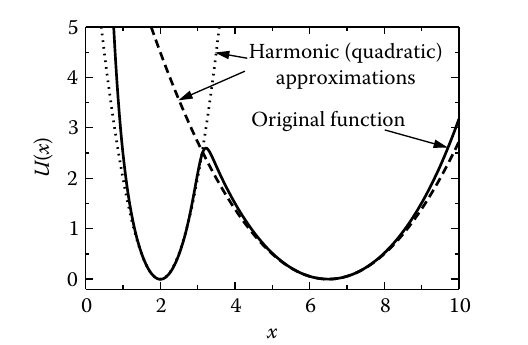
\includegraphics[width=0.7\linewidth]{estados}
\caption{Esquema general en el que se bosquejan dos estados según como se define en este trabajo. A cada uno de ellos se le hace una aproximación como de oscilador armónico ({\color{red} fuente: Zuckerman})}
\label{estados}
\end{figure}

 
 
 \begin{equation}
     P_A=Z^{-1} \frac{1}{h^{3N}} \int_{-\infty}^{\infty}d{\bf p}\int_{V_A}d{\bf x}{\hspace{0.1 cm}}e^{-\frac{E({\bf x},{\bf v})}{K_BT}}
 \end{equation}
 
 Claramente, un resultado absolutamente análogo se tiene para encontrar la probabilidad de encontrar el sistema en el estado B, con la única diferencia de que se cambia el ``volumen" de integración por el correspondiente al del estado B. Ahora, la probabilidad relativa, es:
 
 \begin{equation}\label{prob_rel}
     \frac{P_A}{P_B}=\frac{Z^{-1} \frac{1}{h^{3N}} \int_{-\infty}^{\infty}d{\bf p}\int_{V_A}d{\bf x}{\hspace{0.1 cm}}e^{-\frac{E({\bf x},{\bf v})}{K_BT}}}{Z^{-1} \frac{1}{h^{3N}} \int_{-\infty}^{\infty}d{\bf p}\int_{V_B}d{\bf x}{\hspace{0.1 cm}}e^{-\frac{E({\bf x},{\bf v})}{K_BT}}}=\frac{\frac{1}{\lambda^{3N}}\int_{V_A}d{\bf x}{\hspace{0.1 cm}}e^{-\frac{u({\bf x})}{K_BT}}}{\frac{1}{\lambda^{3N}}\int_{V_B}d{\bf x}{\hspace{0.1 cm}}e^{-\frac{u({\bf x})}{K_BT}}}
 \end{equation}
 
 Nótese que en la última igualación se ha eliminado la función de partición y que así mismo se pudiera haber hecho con la constante $\lambda$, aun así se ha evitado hacerlo porque se busca encontrar una expresión que dé cuenta de la probabilidad relativa de cada estado, la cual debe ser adimensional. Precisamente, a partir de esa expresión se define la energía libre como la cantidad que reemplaza la energía en el factor de Boltzmann y da cuenta de la probabilidad relativa de un estado \cite{zukerman}. En términos matemáticos, esto quiere decir, como se puede inferir de la ecuación  (\ref{prob_rel}), que la energía libre del estado $F_A$ se escribe:
 
 \begin{equation}
     e^{-\frac{F_A}{K_BT}}=\frac{1}{\lambda^{3N}}\int_{V_A}d{\bf x}{\hspace{0.1 cm}}e^{-\frac{u({\bf x})}{K_BT}}
 \end{equation}
 
De aquí se obtiene la definición más común en los textos donde tocan este tema \cite{haile}:

\begin{equation}
    F_A=-K_BT\hspace{0.1 cm}Ln\left(\lambda^{-3N}\int_{V_A}d{\bf x}{\hspace{0.1 cm}}e^{-\frac{u({\bf x})}{K_BT}}\right)=-K_BT\hspace{0.1 cm}Ln\left(Z\right)
\end{equation}

Nótese que, por construcción, ésta definición de energía libre da cuenta de las probabilidades relativas y por lo tanto se puede escribir:

\begin{equation}
    \frac{P_A}{P_B}=\frac{e^{-\frac{F_A}{K_BT}}}{e^{-\frac{F_B}{K_BT}}}=e^{-\frac{(F_A-F_B)}{K_BT}}
\end{equation}

Una vez obtenida una expresión para la energía libre, se puede definir la entropía S como:

\begin{equation}
    S=\frac{\langle E\rangle-F}{T}
\end{equation}

Nótese que ésta definición es totalmente correspondiente con la definición termodinámica de energía libre, $F=\langle E\rangle-TS$, que a su vez implica:

\begin{equation}\label{entropia}
    e^{-\frac{F}{K_BT}}=e^{\frac{S}{K_B}}e^{-\frac{\langle E\rangle}{K_BT}}
\end{equation}

Visto de esta manera, según como hemos desarrollado este marco teórico, se puede obtener una conclusión importante del significado de la entropía desde un punto de vista estadístico. Para ello, nótese que al lado izquierdo de la ecuación (\ref{entropia}) se tiene un término que da cuenta de la probabilidad relativa de un estado, mientras que en el lado derecho se tiene un factor de Boltzmann con la energía media del sistema, es decir, la probabilidad de encontrar el sistema en una configuración correspondiente a la energía media. De manera que el término que contiene la entropía compensa la probabilidad del resto de configuraciones pertenecientes al estado. En otras palabras, la entropía da cuenta de la ``extensión" del estado, que es, la cantidad de configuraciones que pertenecen al estado. Demás interpretaciones similares y más profundas en cuestiones conceptuales y correspondencias físicas se pueden tratar a partir de las definiciones dadas pero están más allá de los intereses de este trabajo.

\subsection{Perfil de energía libre}

En sistemas donde se tiene un gran número de variables (como una proteína por ejemplo), utilizar la definición de densidad de probabilidad mostrada en la ecuación (\ref{densidad_proba}) hace imposible el análisis físico y la identificación de las implicaciones de los resultados que se obtengan dado que hallar una solución analítica en la mayoría de los casos reales es casi imposible y aun con las soluciones numéricas es realmente poca la información directa que se puede obtener dada la complejidad del sistema. En su lugar, lo mejor que se puede hacer es tratar de reducir el sistema a unas cuantas variables que den cuenta de la información que se quiere obtener de un sistema. Más adelante, en este trabajo, se hablará más en detalle sobre éstas variables. Por ahora, se define el perfil de energía libre con respecto a una variable $s= S({\bf x})$ (la mayúscula se usa aquí para denotar la función y la minúscula para la variable) como la proyección de la función de probabilidad sobre esa variable.

\begin{equation}\label{FES}
    e^{-\frac{F(s)}{K_BT}}=P(s)= \frac{Z^{-1}\int d{\bf x}\hspace{0.1 cm}\delta \left(s-S({\bf x})\right)e^{-u({\bf x})/K_BT}}{\rho^{uni}(s)}
\end{equation}

Donde el término $\rho^{uni}(s)$ corresponde a un factor de escala necesario para conservar la norma, las dimensiones y las propiedades del delta de dirac en la variable s, por lo tanto depende del conjunto de variables s que se escojan. Por ejemplo $\rho^{uni}(s)=1/L$ en caso de que $S({\bf x})={\bf r_i}\cdot{\bf i}$, siendo ${\bf i}$ el vector unitario paralelo al eje x, o en otras palabras, s siendo la componente en el eje x de la posición del i-esimo ion, suponiendo que ésta sólo puede variar entre 0 y L.

Esta cantidad es de una relevancia contundente, dado que brinda una forma clara y concisa de analizar sistemas de muchos cuerpos y obtener resultados claros de las configuraciones del sistema. Por ejemplo, tomando s siendo los ángulos diedros en una molécula, se puede encontrar las configuraciones quirales, la probabilidad de las mismas y trazar trayectorias de reacción \cite{laio-gervasio}.

\subsubsection{Variables colectivas}

Como ya se ha dicho, la idea y la ventaja con el perfil de energía libre es reducir la cantidad de variables a aquellas que contengan la información que se esté buscando. El objetivo es entonces encontrar unas variables, a las que se les asignará el nombre de variables colectivas (CVs), lo suficientemente buenas para describir un sistema. Lo que intuitivamente supone un reto fundamental en la construcción de ésta teoría, dado que un error en la elección de éstas podría resultar en una no convergencia del algoritmo o que las conclusiones lleguen a ser erradas. Sin embargo, la experiencia ha arrojado que la elección de unas buenas CVs están ligadas con un conocimiento profundo del sistema a simular \cite{branduardi}, así que la elección de éstas variables no es realmente un problema radicado en el algoritmo de la metadinámica sino que es un asunto más relacionado con el conocimiento {\it a priori} de la evolución del sistema. Por lo tanto, en ocasiones, se opta por hacer simulaciones previas y hacer filtros sobre varias variables hasta escoger las indicadas. 

Además, si bien no se tiene una receta sobre la construcción de las CVs, al menos con el tiempo se han concluido algunas características principales que deben ser cumplidas \cite{barducci}, y éstas son:
\begin{itemize}
    \item Se debe tener claro qué rangos de las CVs escogidas pertenecen a un estado u otro. Además, se deben existir configuraciones posibles entre estados.
    \item Debe contener las variaciones lentas correspondientes a la escala temporal que se esté simulando.
    \item Deben ser una cantidad finita y en lo posible, una baja cantidad. 
\end{itemize}

La primera característica en esta lista surge de la necesidad de construir rutas te reacción entre estados que, se suponen en principio, son suaves con respecto a las variables colectivas. Ésta es una característica para garantizar el significado físico de las variables escogidas.


\begin{figure}[t]
\centering
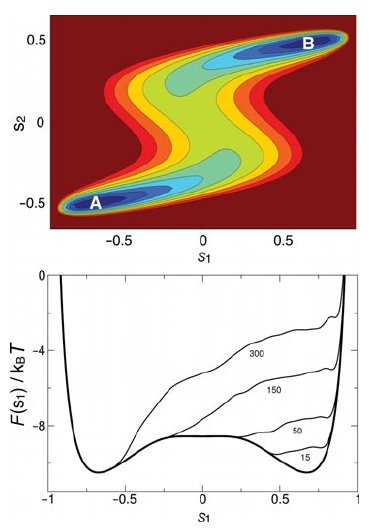
\includegraphics[width=0.6\linewidth]{CVs}
\caption{Ejemplo de lo que puede suceder al usar las CVs inadecuadas, en este caso se muestra en la parte de arriba la superficie de energía libre para dos variables $S_1$ y $S_2$ y en la parte de abajo se muestra el resultado de aplicar metadinámica sobre la variable $S_1$ únicamente.({\color{red} \cite{barducci}})}
\label{error_CV}
\end{figure}

El segundo ítem contemplado, que es de hecho el más complicado, lo que dice precisamente es que tales CVs deben contener la dinámica, considerando que las variaciones rápidas del sistema pueden ser promediadas sin pérdida de generalidad. Sin embargo si no se tienen en cuenta todas las variables que concuerden con los cambios del sistema a la escala temporal escogida, puede suceder algo como lo que se presenta en la Figura \ref{error_CV}, donde se toma un potencial dos dimensional de ejemplo (parte superior) en el que se ve claramente que para pasar del estado A al B, hay que superar barreras para ambas CVs. A partir de ese potencial, se proyecta a lo que sería la energía libre solamente de la CV $s_1$ (línea gruesa) y se trata de hacer el llenado de metadinámica como ya se describió antes, pero únicamente para esa CV (línea delgada). La consecuencia es que el sistema se queda estancado en uno de los estados (el B en la gráfica mostrada) dado que al usar solamente $s_1$ no se está considerando la parte de la dinámica que está escondida en la CV $s_2$, que es muy relevante porque contiene una barrera de energía que evita que el sistema pase de un estado a otro. Así, se presenta un fenómeno de histéresis que se prevé continúe a medida que el llenado se continúa llevando a cabo y provocando que no haya una convergencia en la energía libre.

Finalmente la razón del último ítem citado es sencilla y es la limitada capacidad de computo. Si el número de las variables colectivas es muy grande, los tiempos de llenado de los pozos de energía libre se hacen cada vez más extensos al punto de ser imposible llevar a cabo cálculos de tal magnitud, por lo que la razón de esta condición para las variables colectivas es una cuestión práctica. De manera que se busca obtener información completa del sistema en base a sólo unas cuantas variables.\\

En química usualmente se refieren a éstas variables como variables de reacción. A continuación se presentan sólo un par de ejemplos de las mismas, aunque en la literatura se puede encontrar una gran variedad de éstas \cite{fiorin}.\\

{\bf Variables de relaciones geométricas:} Son aquellas que caracterizan la conformación geométrica de las moléculas. Por ejemplo, éstas variables pueden ser distancias o ángulos formados por tres o más átomos. Éstas variables son las más simples y son ampliamente usadas en biofísica, por ejemplo, para estudiar reconocimiento de proteína-ligante \cite{masetti}.

{\bf Número de coordinación:} Ésta variable mide el número de átomos ligados entré sí. Matemáticamente está definido como:

\begin{equation}
    s({\bf x})=\sum_{i<j}f(r_{i,j})
\end{equation}

con 

\begin{equation}
    f(r)=\frac{1-(r_{ij}/r_0)^n}{1-(r_{ij}/r_0)^m}
\end{equation}

donde i, j corren sobre dos conjuntos de átomos diferentes. En biofísica, ésta variable puede usarse para contar el número de enlaces con hidrógenos \cite{bussi}.

\subsubsection{Cálculo de la energía libre}

Las integrales que aparecen en la ecuación (\ref{FES}) son usualmente difíciles de integrar de forma analítica. Sin embargo, encontrar un resultado numérico para la energía libre no parece ser muy complicado dada su relación con la probabilidad. Básicamente, el proceso consiste en hacer un muestreo del espacio al hacer evolucionar el sistema bajo acción de una dinámica (Newtoniana o de Langevin, por ejemplo), hacer un histograma con las configuraciones encontradas evaluando el valor de $s$ en cada una de ellas y con el histograma obtener una distribución de probabilidad o de forma equivalente, evolucionar el sistema durante un tiempo t y así obtener $P(s)=\frac{1}{t}\int_0^tdt' \delta(S({\bf x}(t'))-s)$. Una vez encontrada ésta distribución, basta con calcular el logaritmo natural, multiplicarlo por $-K_BT$ y listo.

Sin embargo, aunque la descripción anterior del método parezca bastante simple, existen grandes problemas en llevar a cabo el muestreo, ya que por más que se deje evolucionar el sistema, éste se mantendrá confinado en los estados más estables y las configuraciones ``extrañas" no llegan a ser muestreadas. Entonces la superficie de energía libre no queda totalmente reconstruida. Por tal razón, algunos investigadores han trabajado en proponer alternativas y de allí han surgido métodos como por ejemplo {\it umbrela sampling} \cite{patey-valleau}, {\it free energy perturbation} \cite{bash-singh} y metadinámica \cite{laio-gervasio}. En éste trabajo se hará énfasis en éste último método considerando sus ventajas. \\

La idea conceptual sobre la que yace la metadinámica es la de llenar los pozos de energía libre, comenzando desde el punto más profundo del mismo de tal manera que se llegue a un tope lo más pronto posible. Es como si alguien cayera en un hoyo oscuro y no supiera por qué lado queda la salida más cercana. Si escalara por una de las paredes escogida de forma aleatoria, podría irse por aquella que es más alta y quizás no tenga una salida confiable. Entonces decide poner granos de arena sobre el piso y va subiendo el nivel del suelo hasta que llega a un borde. Es posible que el borde de ese pozo, no lo lleve directamente hacia la salida sino que lo lleva a otro pozo sobre el que tendría que hacer lo mismo hasta que llegue a donde espera.

En la práctica, el análogo a poner granos de arena en el método consiste en agregar cada $\tau_G$ pasos temporales una Gaussiana a la energía potencial que hace evolucionar el sistema. De manera que la energía potencial adicional resultante tras $t$ pasos de tiempo está dado por:

\begin{equation}
    V_G(s,t)=\omega\sum_{i=\tau_G,2\tau_G...}^{i<t}e^{-\frac{(s-s(i))^2}{2\delta s^2}}
\end{equation}

 Donde $\omega$ es la altura de la Gaussiana, $\delta s$ es el ancho de la Gaussiana y $\tau_G$ se recuerda que es la periodicidad con la que se agrega una nueva Gaussiana. Entonces, a la energía potencial del sistema se le agrega $V_G$ como valor adicional, el cual claramente no hace parte de la dinámica normal de el sistema sino que es un término agregado meramente para acelerar el muestreo del sistema y por lo tanto las fuerzas atómicas cambian a ser:
 \begin{equation}\label{forces}
    {\bf f_i}({\bf x})=-\frac{\partial u({\bf x})}{\partial {\bf r_i}}-\frac{\partial V_G(s)}{\partial s}\frac{\partial s}{\partial {\bf r_i}}
\end{equation}

Para llevar a cabo la evolución, se puede por ejemplo, aplicar recursivamente una ecuación de Langevin sobreamortiguado  \cite{zukerman} la cual es de la forma:

\begin{equation}
    \frac{d{\bf r_i}}{dt}=-\frac{1}{m\gamma}{\bf f_i}+\frac{1}{m\gamma}{\bf f_{rand}}
\end{equation}

Donde el primer término ${\bf f_i}$ contiene tanto las fuerzas de las interacciones típicamente usadas en las simulaciones de dinámica molecular como la fuerza adicionada correspondiente a la metadinámica tal como se ve en (\ref{forces}), mientras que ${\bf f_{rand}}$ supone una fuerza térmica que se incrementa con la temperatura.\\

Y es de ésta manera que al sistema se le van inyectando de forma suave impulsos para explorar nuevas configuraciones posibles en el sistema y así reconstruir el perfil de energía libre.\\

Transcurrido una cantidad de pasos de tiempo suficientes se puede demostrar que \cite{PRL_Bussi}:

\begin{equation}
     \lim_{t\to\infty}V_G(s,t)=-F(s)
\end{equation}



\begin{figure}[t]
\centering
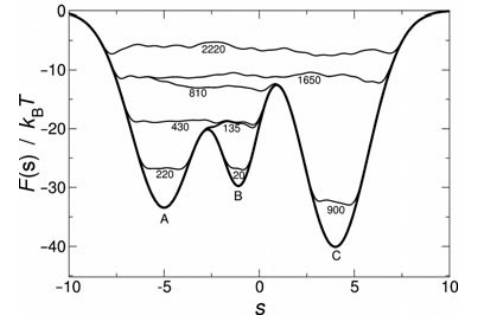
\includegraphics[width=0.7\linewidth]{evolution}
\caption{Ejemplo de evolución de la construcción de la energía libre. Nótese que se parte del pozo de la mitad y en el paso de tiempo 135 llega al borde donde cae al pozo más accesible energéticamente. Sigue evolucionando y llega, en el paso 810, al pico energético más cercano y cae de nuevo a otro pozo. Así se procede hasta llegar obtener un buen mapeo del sistema en cuestión. ({\color{red}\cite{barducci}})}
\label{ejemplo_muestreo}
\end{figure}

En la figura \ref{ejemplo_muestreo} se puede apreciar un ejemplo de evolución con metadinámica. De allí se puede notar que al final de la simulación, la aproximación que se ha hecho a la energía libre puede contener cierta cantidad de ruido. Como se puede intuir, entre mayor sea la altura de las gaussianas, el llenado de los pozos se llevará a cabo en un tiempo menor, pero será mayor el ruido al final y por lo tanto el error. En contraposición, si se escoge una altura pequeña en comparación con la profundidad de los pozos de energía libre, se obtendrá una mejor aproximación, pero la simulación tardaría muchísimo más. Una forma de reducir este problema es tomar varios muestreos y promediarlos. Explícitamente, el error que se obtiene en cada corrida del algoritmo es \cite{barducci}:

\begin{equation}
    \epsilon \propto\sqrt{\frac{\omega K_BT}{D\tau_G}}
\end{equation}

Donde D es el coeficiente de difusión intrínseco del sistema. Nótese que además de las anotaciones que se habían hecho sobre el error, surge una adicional que es la dependencia con $\tau_G$. Para lograr un resultado con un error menor hay que procurar fijar el $\tau_G$ grande, lo que implica también un tiempo de simulación mayor para poder alcanzar un llenado completo de los pozos de energía libre.\\

A propósito del tiempo necesario para completar el llenado de los pozos, éste aspecto es un tanto incomodo para la metadinámica como se ha descrito hasta ahora, dado que no se tiene un criterio claro para definir la suficiencia en la cantida de gaussianas agregadas y acarrea consigo también el riesgo de que el sistema decaiga y se estanque en regiones de CVs irrelevantes físicamente.

Para contrarrestar éste pequeño problema ha surgido un método alternativo llamado {\it well-tempered metadynamics}  \cite{wellmeta} que varía un poco el algoritmo original y consiste en hacer que el tamaño de la altura de las gaussianas agregadas sean decrecientes en el tiempo. Con éste cambio, la energía adicional al sistema original resulta siendo:

\begin{equation}
     V_G(s,t)=\sum_{i=1}^{i<t/\tau_G}\omega e^{-\frac{V_G(s,t)}{K_B\Delta T}}e^{-\frac{(s-s(i \tau_{\small{G}}))^2}{2\delta s^2}}
\end{equation}

 Donde $\Delta T$ es un parámetro que se puede fijar según se considere. Nótese que al agregar éste térimino se logra que las gaussianas agregadas sean menores dependiento estrictamente de la cantidad de las agregadas anteriormente sobre el mismo punto de la variable colectiva. 
 
 Con esta modificación se logra que toda simulación converja al mismo valor que ahora estará dado por:
 
 \begin{equation}\label{VFwellmeta}
     V_G(s,t\rightarrow\infty)=-\frac{\Delta T}{T+\Delta T} F(s)
 \end{equation}

Nótese que de la ecuación (\ref{VFwellmeta}) se puede concluir que tomando $\Delta T\rightarrow0$ se tiene el algoritmo de dinámica molecular estándar. Por otra parte, si se toma $\Delta T\rightarrow\infty$ se recupera el algoritmo de metadinámica sin modificaciones.
















\vspace{20 cm}

Comentarios:

- ¿Será que hablo de la idea de Thomas-Fermi para ejemplificar la idea inicial de trabajar con densidades? R: No es realmente necesario, si se tiene tiempo y se quiere ampliar un poco, se podría agregar sin tener que ahondar mucho. A menos que sobre tiempo podría agregarse como un bonus





















 

























\vspace{20 cm}
\nocite{*}
\bibliographystyle{IEEEannot}
\bibliography{annot}
\end{document}